\section{Overview}

\begin{frame}
\frametitle{Today's Goals}
\begin{itemize}
	\visible<1->{\item Overview of ROS}
	\visible<2->{\item Using built-in ROS tools}
	\visible<3->{\item Writing custom ROS nodes}
\end{itemize}
\end{frame}

\begin{frame}
\frametitle{Today's Overview}
\begin{itemize}
	\visible<1->{\item 9:00 What is ROS and why do we want it}
	\visible<3->{\item 10:30 Coffe Break}
	\visible<2->{\item 10:45 Start with the ROS tutorials}
	\visible<3->{\item 12:30 Lunch Break}
	\visible<4->{\item 13:30 Continue with the ROS Tutorials}
	\visible<5->{\item 14:45 Coffee Break}
	\visible<6->{\item 15:00 Build a ROS node which uses deep learning to process MNIST images}
	\visible<7->{\item 16:00 Small ROS Quiz: Use the ROS tools on a Rosbag from the RC-Car}
	\visible<8->{\item 17:00 Checking who Survived :P}
\end{itemize}
\end{frame}

\section{Introduction to ROS}
\begin{frame}
\frametitle{Building a Robot}
\visible<1->{
\begin{itemize}
	\visible<1->{\item{Without ROS
		\visible<2->{
			\begin{itemize}
				\item{Build device drivers}
			\visible<3->{\item{Build a communications framework}}
			\visible<4->{\item{Write algorithms for perception, navigation, motion planning,…}}
			\visible<5->{\item{Implement logging, control and error handling}}
			\end{itemize}
		}
	}}
	\visible<6->{\item{With ROS
		\visible<7->{
			\begin{itemize}
				\item{Logging, error handling, communications framework, driver for standard devices and even some perception, navigation and motion planning algorithms are already provided.}
			\visible<8->{\item{There is a package management system included, making the development way easier.}}
			\visible<9->{\item{It provides tools for visualisation, simulation and analysis}}
			\end{itemize}
		}
	}}
	\end{itemize}
		}

\end{frame}


\begin{frame}
\frametitle{History of ROS}
\visible<1->{
\begin{itemize}
	\item{Development started in 2000 in the Stanford Artificial Intelligence Lab as project Switchyard.}
	\visible<2->{\item{In 2007 it became a formal entity with support from Willow Garage.}}
	\visible<3->{\item{Since 2013 the Open Source Robotics Foundation is maintaining and developing ROS.}}
	\visible<4->{\item{The primary motivation behind ROS was the recognition that researchers were constantly reinventing the wheel as there were no reusable components for robotics projects to start from.}}
	\visible<5->{\item{In addition, it was hard for researchers to exchange and validate code from other researchers.}}
\end{itemize}
}

\end{frame}

\begin{frame}
\frametitle{High Level Robot Tasks}
\begin{figure}[h]
	\begin{tikzpicture}[scale=.55]
		\definecolor{lightblue}{rgb}{.2,.6,1}
		\definecolor{lightred}{rgb}{.8,.2,.2}
		\definecolor{lila}{rgb}{.6,.2,.6}
		\visible<2->{\pgftext{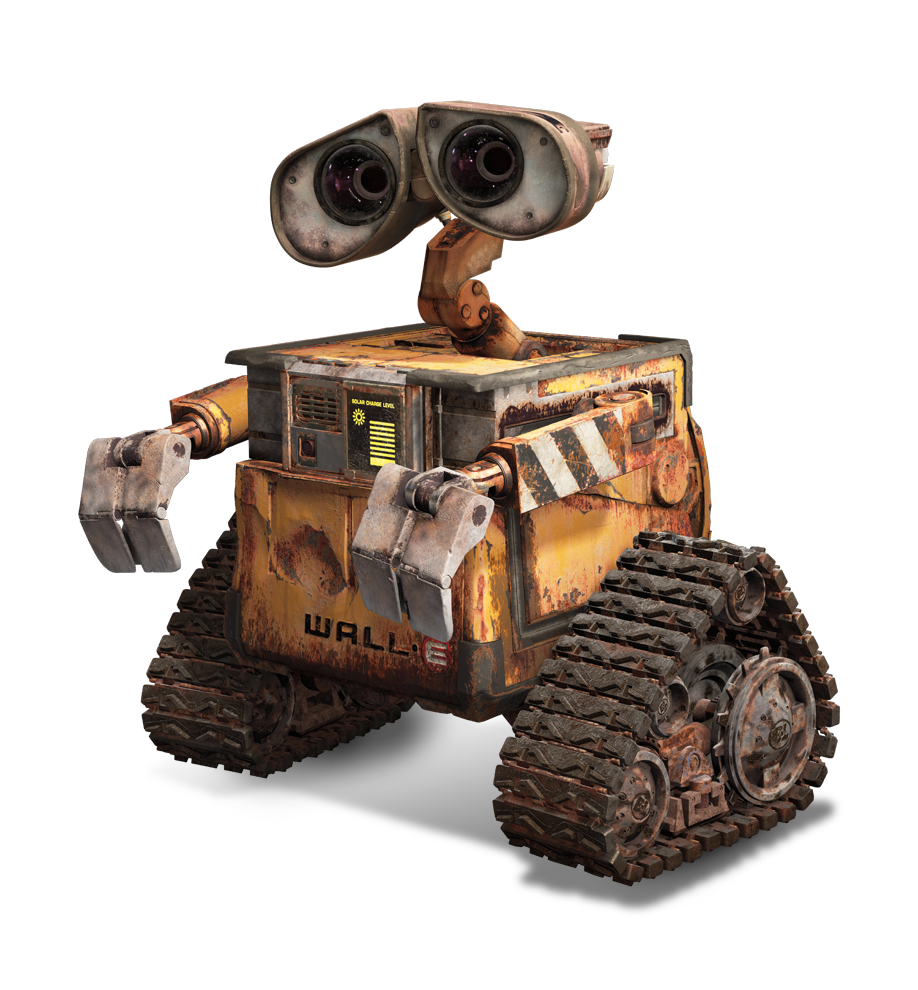
\includegraphics[width=150pt]{./figs/Wall-E.png}} at (-5,0);}
		\visible<3->{\coordinate (Perception) at (8,7);
		\fill[fill=lila, opacity = .7] (Perception) ellipse (3 and 1);
		\draw (Perception) node{Perception};}
		\visible<4->{\coordinate (Decision Making) at (8,3.5);
		\fill[fill=lightred, opacity = .7] (Decision Making) ellipse (3 and 1);
		\draw (Decision Making) node{Decision Making};}
		\visible<5->{\coordinate (Actuation) at (8,0);
		\fill[fill=yellow, opacity = .7] (Actuation) ellipse (3 and 1);
		\draw (Actuation) node{Actuation};}
		\visible<6->{\draw[->, line width=2mm] (Perception) ++ (0,-1.1) -- ++(0,-1.3);}
		\visible<7->{\draw[->, line width=2mm] (Decision Making) ++ (0,-1.1) -- ++(0,-1.3);}
	\end{tikzpicture}
\end{figure}
\visible<7->{Literally every robot is performing these high level tasks.}
\end{frame}

\begin{frame}
\frametitle{Nodes}
\visible<1-7>{ROS splits these high level tasks in low level ones and spawns a unix thread for each of them.}
\visible<2-7>{\begin{figure}[h]
	\begin{tikzpicture}[scale=.55]
		\definecolor{lightblue}{rgb}{.3,.7,1}
		\definecolor{lightred}{rgb}{.8,.2,.2}
		\definecolor{lila}{rgb}{.6,.2,.6}
		\definecolor{grey}{rgb}{.4,.4,.4}
		\definecolor{darkgrey}{rgb}{.3,.3,.3}
		\coordinate (Perception) at (5,9);
		\fill[fill=grey, opacity = .7] (0,0) -- (0,10) -- (10,10) -- (10,0) -- cycle;
		\draw[white] (Perception) node{Perception};
		\coordinate (Decision Making) at (13,9);
		\fill[fill=darkgrey, opacity = .7] (10,0) -- (10,10) -- (16,10) -- (16,0) -- cycle;
		\draw[white] (Decision Making) node{Decision Making};
		\coordinate (Actuation) at (19,9);
		\fill[fill=grey, opacity = .7] (16,0) -- (16,10) -- (22,10) -- (22,0) -- cycle;
		\pgftext{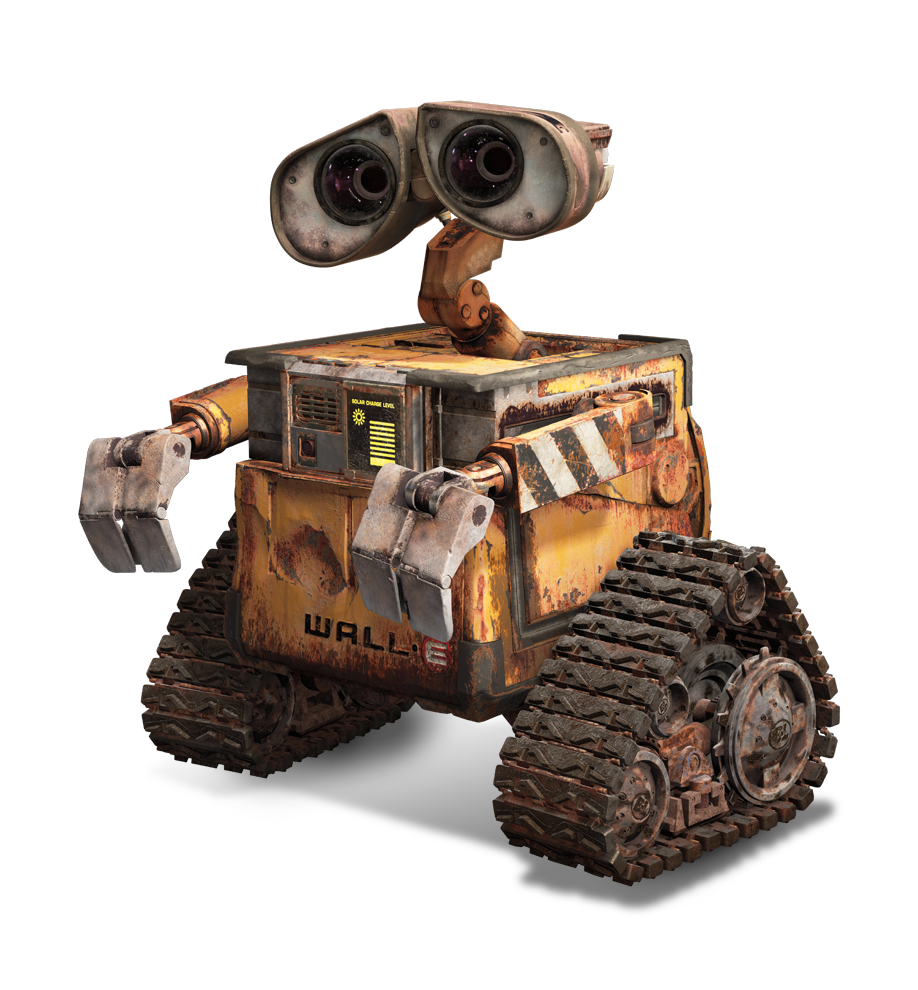
\includegraphics[width=150pt]{./figs/Wall-E.png}} at (10,3);
		\draw[white] (Actuation) node{Actuation};
		\visible<3->{\coordinate (Wheel Encoder) at (3,7);
		\draw[white, fill=lightblue, opacity = .7] (Wheel Encoder) ellipse (2.5 and 1);
		\draw (Wheel Encoder) node{Wheel Encoder};}
		\visible<4->{\coordinate (Camera) at (3,4.5);
		\draw[white, fill=lightblue, opacity = .7] (Camera) ellipse (2.5 and 1);
		\draw (Camera) node{Camera};}
		\visible<5->{\coordinate (Position Estimation) at (3,2);
		\draw[white, fill=lightblue, opacity = .7] (Position Estimation) ellipse (2.5 and 1);
		\draw (Position Estimation) node{Position Estimation};}
		\visible<6->{\coordinate (Behaviour Execution) at (13,7);
		\draw[white, fill=lightblue, opacity = .7] (Behaviour Execution) ellipse (2.5 and 1);
		\draw (Behaviour Execution) node{Behaviour Execution};}
		\visible<7->{\coordinate (Motor Control) at (19,7);
		\draw[white, fill=lightblue, opacity = .7] (Motor Control) ellipse (2.5 and 1);
		\draw (Motor Control) node{Motor Control};}
	\end{tikzpicture}
\end{figure}}
\end{frame}

\begin{frame}
\frametitle{Nodes}
\visible<1->{The ROS Master Process is keeping a registry of all spawned nodes and allows them to establish communication between each other.}
\visible<1->{\begin{figure}[h]
	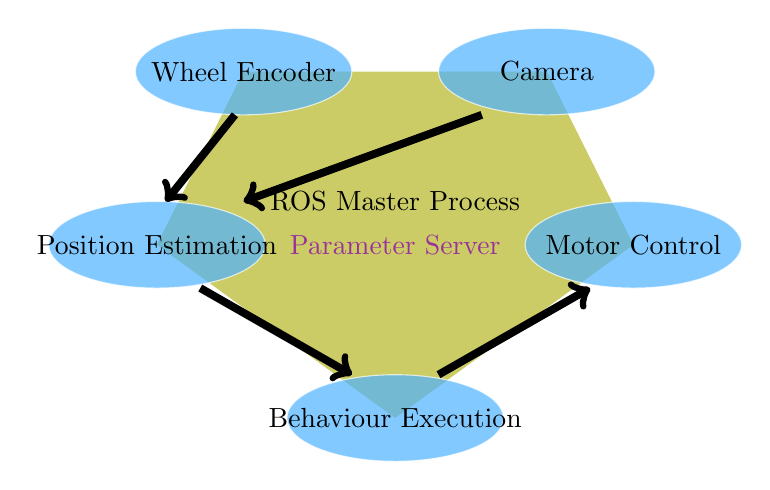
\begin{tikzpicture}[scale=.55]
		\definecolor{lightblue}{rgb}{.3,.7,1}
		\definecolor{lightred}{rgb}{.8,.2,.2}
		\definecolor{lila}{rgb}{.6,.2,.6}
		\definecolor{grey}{rgb}{.4,.4,.4}
		\definecolor{darkgrey}{rgb}{.3,.3,.3}
		\definecolor{lightbrown}{rgb}{.8,.8,.4}
		\coordinate (Wheel Encoder) at (1,7);
		\coordinate (Camera) at (8,7);
		\coordinate (Position Estimation) at (-1,3);
		\coordinate (Motor Control) at (10,3);
		\coordinate (Behaviour Execution) at (4.5,-1);
		\fill[lightbrown] (Wheel Encoder) -- (Camera) -- (Motor Control) -- (Behaviour Execution) -- (Position Estimation) --cycle ;
		\draw (4.5,4) node{ROS Master Process};
		\draw[white, fill=lightblue, opacity = .7] (Wheel Encoder) ellipse (2.5 and 1);
		\draw (Wheel Encoder) node{Wheel Encoder};
		\draw[white, fill=lightblue, opacity = .7] (Camera) ellipse (2.5 and 1);
		\draw (Camera) node{Camera};
		\draw[white, fill=lightblue, opacity = .7] (Position Estimation) ellipse (2.5 and 1);
		\draw (Position Estimation) node{Position Estimation};
		\draw[white, fill=lightblue, opacity = .7] (Behaviour Execution) ellipse (2.5 and 1);
		\draw (Behaviour Execution) node{Behaviour Execution};
		\draw[white, fill=lightblue, opacity = .7] (Motor Control) ellipse (2.5 and 1);
		\draw (Motor Control) node{Motor Control};
		\visible<2->{\draw[->, line width=1mm] (Wheel Encoder) ++(-.2,-1) -- (-.8,4);
			\draw[->, line width=1mm] (Camera) ++(-1.5,-1) -- (1,4);
		}
		\visible<3->{\draw[->, line width=1mm] (Position Estimation) ++(1,-1) -- (3.5,0);}
		\visible<4->{\draw[->, line width=1mm] (Behaviour Execution) ++(1,1) -- (9,2);}

		\visible<5->{\draw[lila] (4.5,3) node{Parameter Server};}
	\end{tikzpicture}
\end{figure}}
\end{frame}

\begin{frame}
\frametitle{Topics}
\begin{itemize}
\visible<1->{\item ROS nodes communicate with each other over topics.}
\visible<2->{\item If they want to send messages, they publish to a topic.}
\visible<3->{\item If they want to receive messages, they subscribe to a topic.}
\end{itemize}

\visible<1->{\begin{figure}[h]
	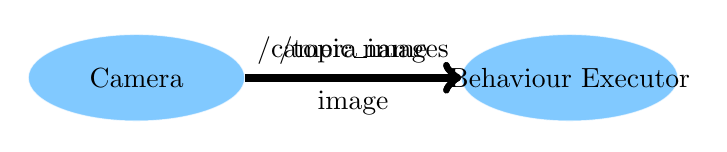
\begin{tikzpicture}[scale=.55]
		\definecolor{lightblue}{rgb}{.3,.7,1}
		\definecolor{lightred}{rgb}{.8,.2,.2}
		\definecolor{lila}{rgb}{.6,.2,.6}
		\definecolor{grey}{rgb}{.4,.4,.4}
		\definecolor{darkgrey}{rgb}{.3,.3,.3}
		\definecolor{lightbrown}{rgb}{.8,.8,.4}
		\coordinate (a) at (0,0);
		\coordinate (b) at (10,0);
		\visible<1-3>{\draw[->, line width=1mm, decorate] (a) ++(2.5,0) -- node[above]{/topic\_name} (7.5,0);}
		\visible<2->{\draw[white, fill=lightblue, opacity = .7] (a) ellipse (2.5 and 1);}
		\visible<3->{\draw[white, fill=lightblue, opacity = .7] (b) ellipse (2.5 and 1);}
		\visible<4->{\draw[->, line width=1mm, decorate] (a) ++(2.5,0) -- node[above]{/camera\_images} node[below]{image} (7.5,0);}
		\visible<4->{\draw (a) node{Camera};}
		\visible<4->{\draw (b) node{Behaviour Executor};}
	\end{tikzpicture}
\end{figure}}
\end{frame}



\begin{frame}
\frametitle{Messages}
\begin{itemize}
\visible<1->{\item ROS comes with a variety of predefined messages for:}
\visible<2->{\item Physical properties, e.g. positions, velocities, acceleration, rotations, durations}
\visible<3->{\item Sensor reading, e.g. laser scans, images, point clouds, inertial measurements}
\visible<4->{\item There are over 200 different message types, but there is still the possibility to define custom ones}
\end{itemize}
\end{frame}

\section{ROS Tutorials}
\begin{frame}
\frametitle{ROS Tutorials}
\begin{center}
Let's get our hands dirty and our fingers on the keyboard. \\
\href{http://wiki.ros.org/ROS/Tutorials}{ROS Tutorial}
\end{center}
\end{frame}

\section{Racecar hacking}
\begin{frame}
\frametitle{Some Notes}
\begin{itemize}
\visible<1->{\item The racecar should stop around 60cm in front of walls. \visible<2->{(theoretically!)}}
\visible<3->{\item Please open and close only the orange connectors.}
\visible<4->{\item The speed is currently limited to 2m/s. \visible<5->{(currently ;))}}
\end{itemize}
\end{frame}















